\subsection{MySQL Adapter}
One way to address the drawbacks of the trigger-based approach is to interact directly with the transaction log, since that does not take up resources on the source database.
Oracle and MySQL both have binary logs that contain the log of changes as they are applied to the database. However, it is fragile to mine these logs and reverse-engineer the structure, because there is no guarantee that the format will be stable across multiple versions. In the case of MySQL though, it is possible to tap into the Storage Engine API. This is a stable interface that has been used to build many commercial and open-source storage engines for MySQL.

%The trigger based approach used by the Oracle Adapter guarantees that every poll issued to the database returns the latest state of every changed row. But it does not guarantee that every change made to that row in that duration is returned to the Adapter. In most cases, this is acceptable but in some usecases, it is desirable to make every change to the row available to the consumer. Another disadvantage of the trigger based approach is the additional load it puts on the source database. If the source database itself maintains a change log which can be read externally, that is a more efficient way for the adapter to pull the change log. In case of Oracle, the redo log is in a proprietary format and cannot be read externally unless Oracle's internal format is reverse engineered. MySQL on the other hand maintains a binary log of changes made to the database which is used by MySQL replication to replicate the changes between MySQL databases.

However, MySQL replication works only between MySQL databases and does not make the change log available to external applications. The pluggable storage engine layer allows MySQL replication to be setup between MySQL databases that might use different storage engines. 
%However, MySQL has a very elegant pluggable architecture that allows multiple storage engines to be plugged in using a common Storage Engine API. This feature of MySQL has created a thriving ecosystem of storage engines include MyISAM, InnoDB, PBXT, Tokutech etc. This feature allows MySQL replication to be setup between MySQL databases that might use different storage engines. 
Thus, a MySQL server using InnoDB storage engine can replicate to MySQL server using the MyISAM storage engine. MySQL replication takes care of the protocol between master and slave, handling restarts across failures, parsing of the binary log and then calling the appropriate insert, update, delete statements on the slave through the storage engine API. Databus uses this feature of MySQL and obtains the change log from the MySQL master into a custom light-weight storage engine RPL\_DBUS that writes to the in-memory log. This architecture is shown in Figure~\ref{fig:mysql-adapter}. The relay manages the local slave MySQL instance and uses MySQL admin commands to connect to the MySQL master.

\begin{figure}
\centering
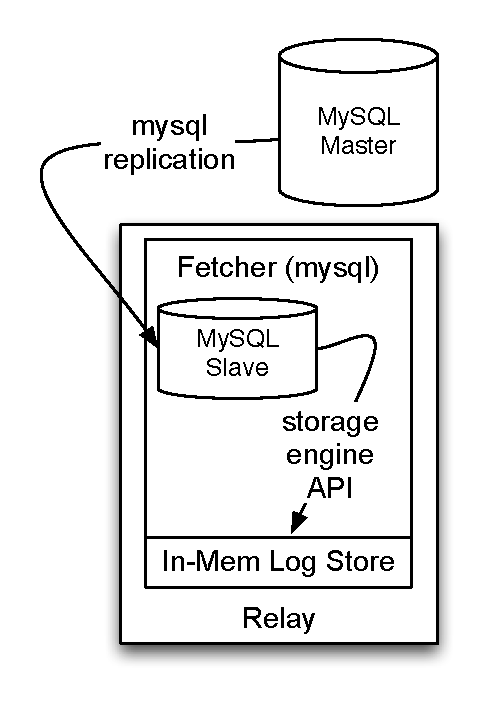
\epsfig{file=figures/mysql-adapter.eps, scale=0.4}
\caption{MySQL Adapter}
\label{fig:mysql-adapter}
\end{figure}
